%\section{Controller tuning}
%\label{sec:PID}
\section{Ziegler-Nichols metode}
Til bestemmelsen af regulator-koefficienterne bruges den analytiske fremgangsmåde "Ziegler-Nichols Tuning Methode", \citep[Kap. 7.6]{reg_modern_control_systems}. 
Metoden tager udgangspunkt i systemets lukket sløjfe respons. 

Tabel \ref{tb:ZieglerNichols} beskriver hvordan regulator-koefficienterne bestemmes.

\begin{figure}[th!]
\centering
\begin{tabular}{c|c|c}
\(K_p\) & \(K_i\) & \(K_d\)\\\hline
\(0,5  { K }_{ U }\) &-&-\\
\(0,45  { K }_{ U }\) & \( \frac { 0,54  { K }_{ U } }{ { T }_{ U } }  \) &-\\
\(0,6  { K }_{ U } \) &  \( \frac { 1,2  { K }_{ U } }{ { T }_{ U } }  \) & \(\frac { 0,6  { K }_{ U }  { T }_{ U } }{ 8 }  \)
\end{tabular}
\captionsetup{type=table}
\caption[Ziegler-Nichols Tuning Methode]{Analytisk fremgangsmåde. "Ziegler-Nichols Tuning Methode".}
\label{tb:ZieglerNichols}
\end{figure}

hvor \(K_U\) er forstærkningen og \(T_U\) er den tilhørende oscillations periode hvorved lukket sløjfe systemet opnår marginalt stabilitiet.

\subsubsection{Pan- og tilt controller-keofficienter}
\(K_u\) og \(T_u\) er bestemt ud fra hhv. pan og tilts diskretiserende overføringsfunktioner, ligning \ref{eq:pantiltdiskretiserendetf}. 
Der blev lavet et loop i MATLAB, som løb forstærkningsintervallet igennem for de to transferfunktioner.
\begin{itemize}
\itemsep1pt
\item \(K_{u-tilt} = 37,24\)
\item \(T_{u-tilt} = 29,917 \cdot 10^{-3}\) [s] 
\item \(K_{u-pan} = 37,12\)
\item \(T_{u-pan} = 34,207\cdot 10^{-3}\) [s] 
\end{itemize}

Regulator-koefficienterne bestemt ud fra den ultimative forstærkning og tilhørende periode, ses i tabel \ref{tb:ZieglerNichols1}.

\begin{figure}[th!]
\centering
\begin{tabular}{c|c|c|c|c|c|c}
&\(K_{p-tilt}\) & \(K_{i-tilt}\) & \(K_{d-tilt}\)&\(K_{p-pan}\) & \(K_{i-pan}\) & \(K_{d-pan}\)\\\hline
P&\(18,62\) &-&-&\(18,56\)&-&-\\
PI&\(1675,8\) & \( 672,1797\) &-&\(1670,4\) & \( 585,9853  \) &-\\
PID&\(22,3440 \) &  \( 1493,7 \) & \(0,0836  \)&\(22,2720 \) &  \( 1302,2 \) & \(0,0952  \)
\end{tabular}
\captionsetup{type=table}
\caption[Controller-koefficienter, Ziegler-Nichols Tuning Methode]{Controller-koefficienter for pan og tilt.}\label{tb:ZieglerNichols1}
\end{figure}

Disse koefficienter ville skabe meget overshoot som vil skade systemet. Systemet er ikke testet med disse koefficienter. 
Istedet er der ved brug af PID tool og simulink i matlab fundet frem til nogle koefficienter.
Disse koefficienter er testet og plottet i Figur \ref{PID_test14_plot} 
\begin{figure}
\centering
  \begin{tabular}{lccc}
      & P & I & D\\
tilt  & 74.4933 & 435.0662 & 0.248960\\
pan   & 37.1740 &  33.3610 & 0.215658
  \end{tabular}
\captionsetup{type=table}
\caption[Regulator koefficienter brugt i test]{Regulator koefficienter brugt til test af system.}
\label{PID_test14} 
\end{figure}

\begin{figure}
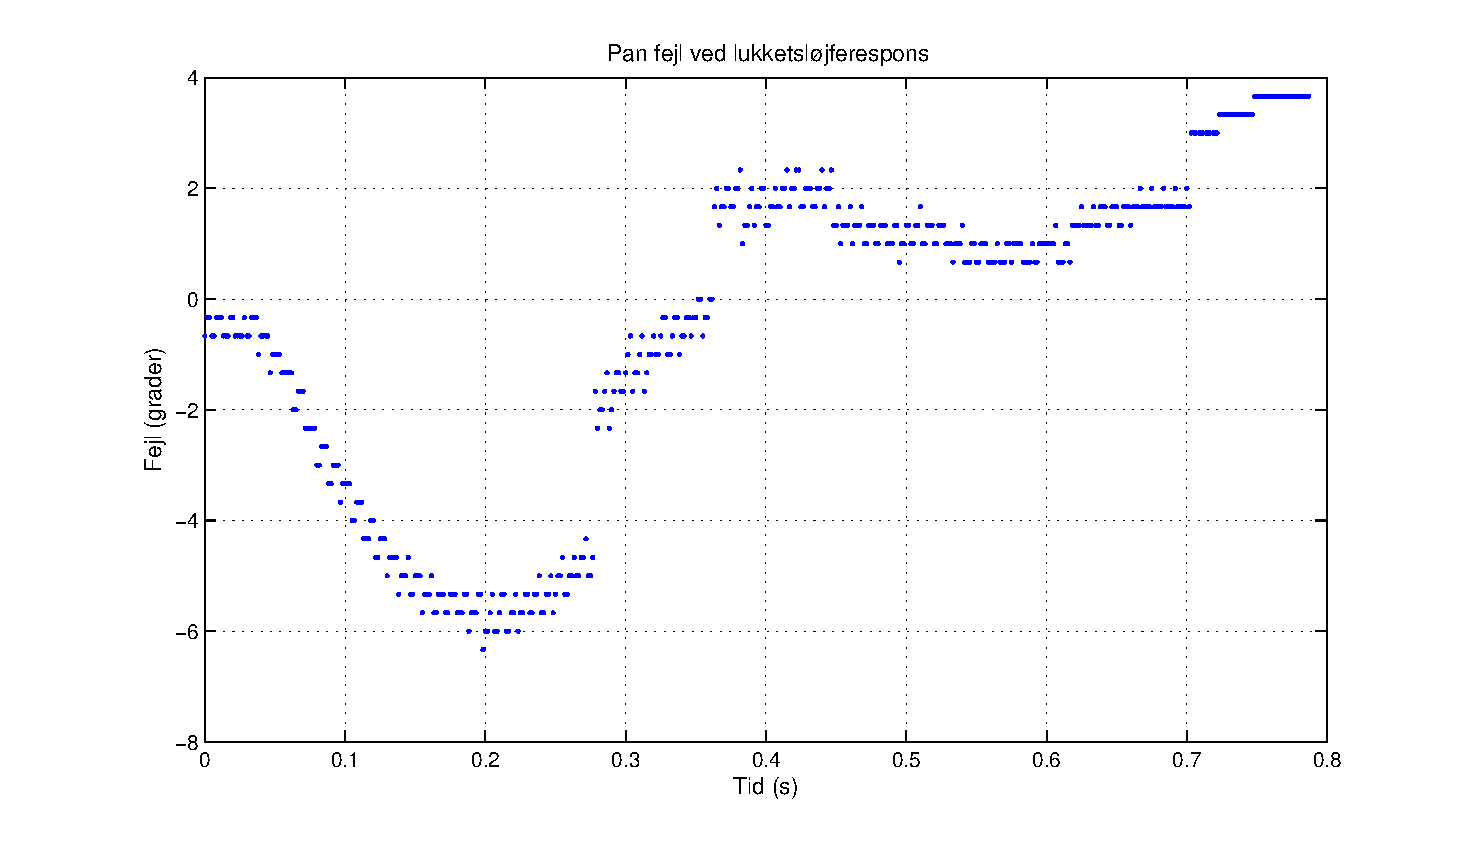
\includegraphics[width=1\textwidth]{./graphics/error_pan.eps}
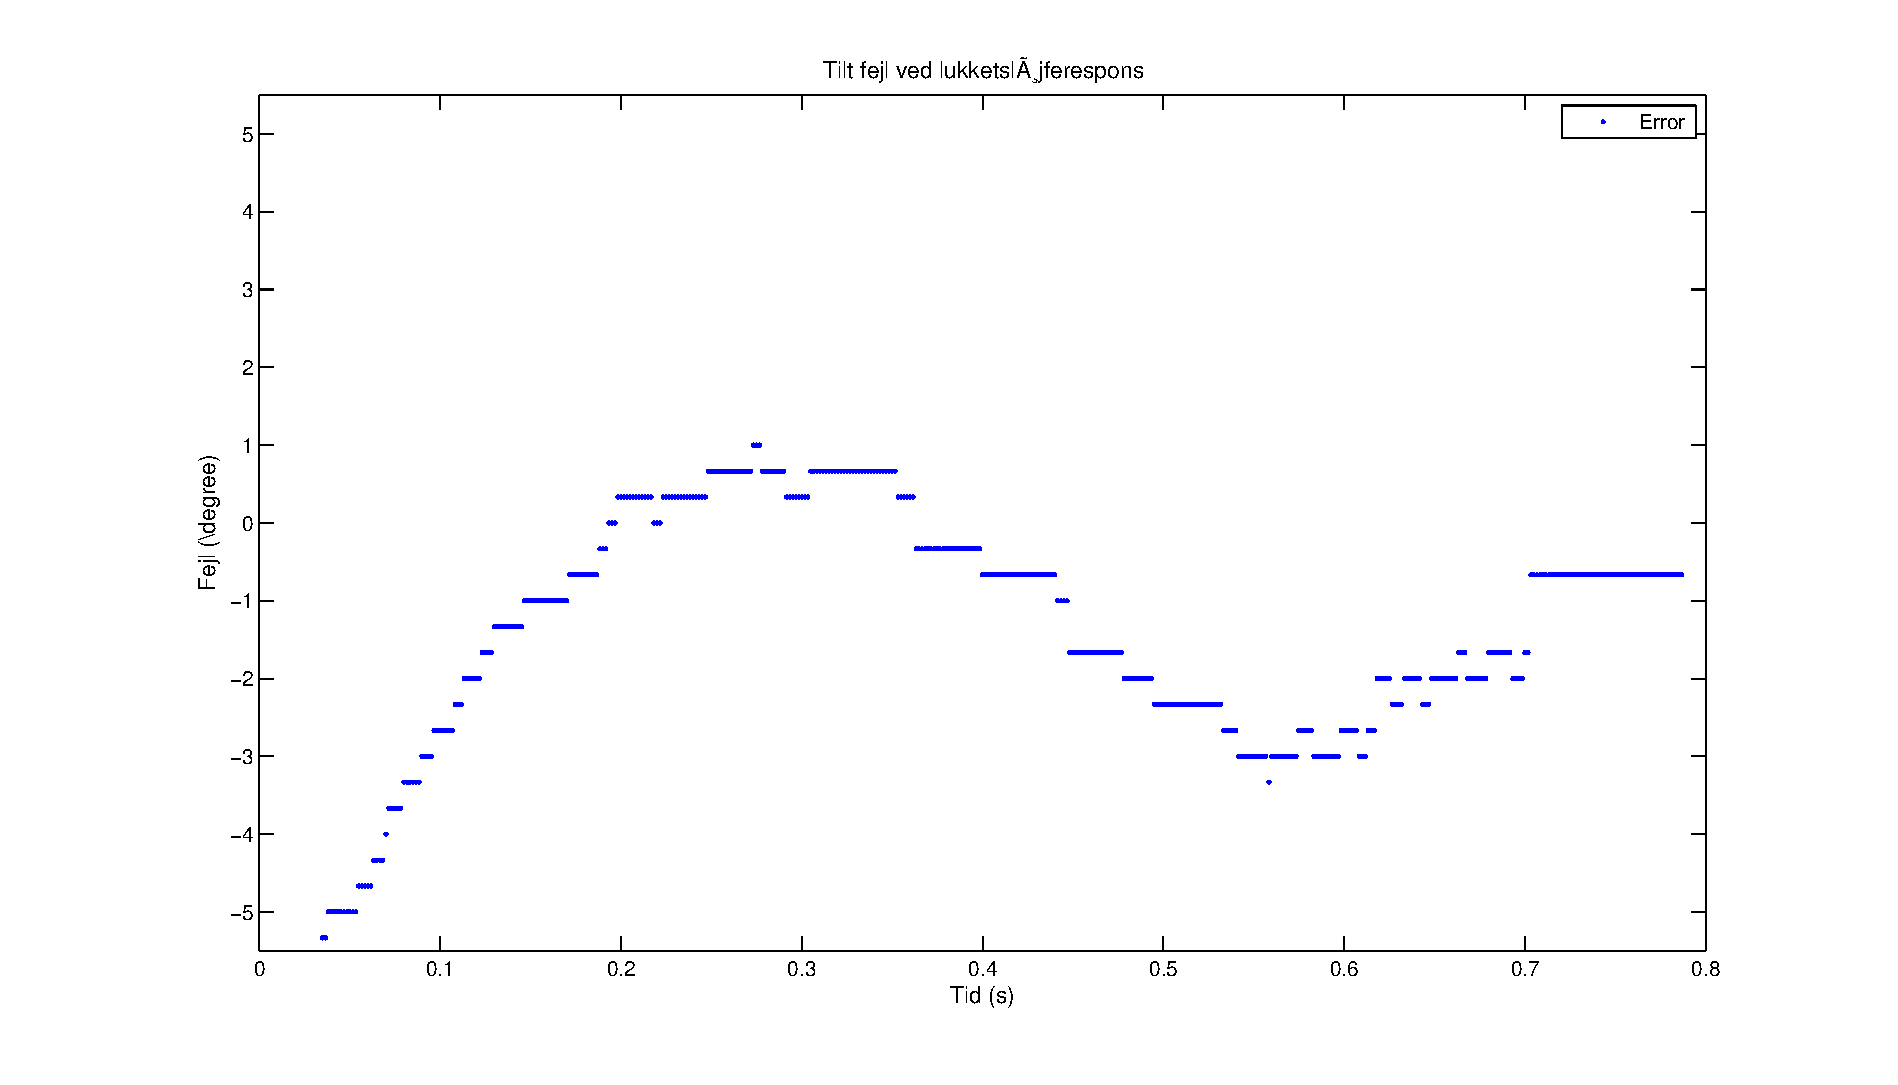
\includegraphics[width=1\textwidth]{./graphics/error_tilt.eps}
\caption{fejl målt i grader for PID controller med coefficienterne beskrevet i Tabel \ref{PID_test14} \label{PID_test14_plot} }
\end{figure}

\subsection{Optimering af controller/koefficienter}